\documentclass[11pt]{article}
\usepackage[run,nohup,julia,cache,stopserver]{code/runcode}
\usepackage{booktabs,float,hyperref}
\newcommand{\due}{1: Solution}

\title{A mini example of calling Julia code from LaTex}

\begin{document}
\maketitle
\section{Some useful commands in Julia REPL}

\begin{itemize}
\item ? (enters help mode);
\item ; (enters system shell mode);
\item ] (enters package manager mode);
\item Ctrl-c (interrupts computations);
\item Ctrl-d (exits Julia);
\item Ctrl-l clears screen;
\item putting ; after the expression will disable showing its value in REPL.
\end{itemize}
\section{Examples code}

Loops and comprehensions rebind variables on each iteration, so they are 
safe to use then creating closures in iteration:
\showCode{julia}{code/samplecode.jl}[8][12]
\runJulia{code/samplecode.jl}{res1}
The above code gives the following output
\includeOutput{res1}

There are several plotting packages for Julia like Plots.jl (which is
an umbrella packages for several plotting backends). Here we show how to use it.
The following code
\showCode{julia}{code/samplecode.jl}[1][6]
creates the following plot.
\begin{center}
  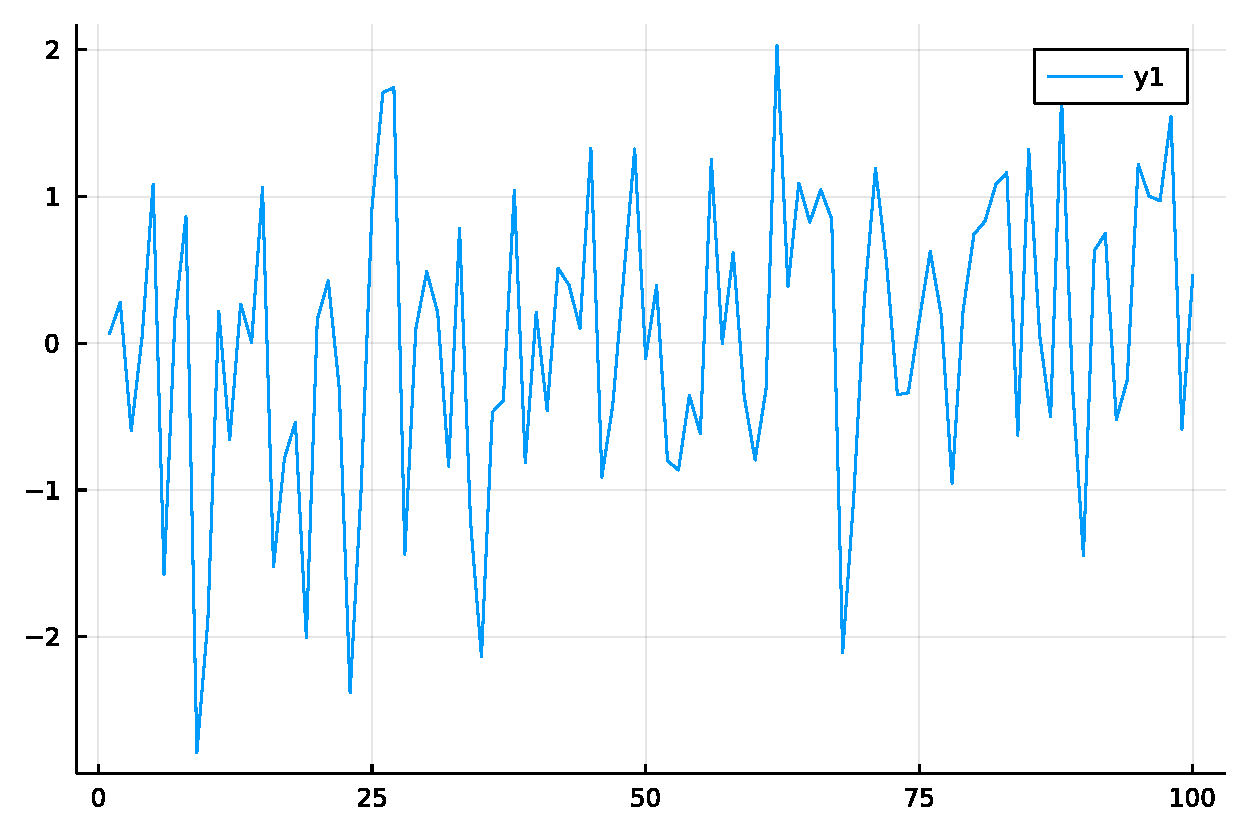
\includegraphics[width=0.75\textwidth]{./tmp/randomplot.pdf}
\end{center}

You can also use the result inline: the sum of $X$ is $\sum_{i=1}^nx_i=$ \inlnJulia{```print(sum(x))```}.

\section{An example of including a table}
There are multiple packages supporting tabular data for the Julia language.
Here we will show how DataFrames.jl package can be used.
Table~\ref{table:1} is created from the following code.

\showCode{julia}{code/table1.jl}[1][5]
\runJulia{code/table1.jl}{table}
\begin{table}[H]
  \centering
  \includeOutput{table}[tex]
  \caption{A sample table.}
\label{table:1}
\end{table}

You may refer to the \href{https://github.com/korsbo/Latexify.jl}{Latexify.jl} package to learn more on how to generate LaTeX formatted strings from julia objects.

\end{document}